\documentclass[%
 reprint,
%superscriptaddress,
%groupedaddress,
%unsortedaddress,
%runinaddress,
%frontmatterverbose, 
%preprint,
%preprintnumbers,
%nofootinbib,
%nobibnotes,
%bibnotes,
 amsmath,amssymb,
 aps,
%pra,
%prb,
%rmp,
%prstab,
%prstper,
%floatfix,
]{revtex4-2}

\usepackage{graphicx}% Include figure files
\usepackage{dcolumn}% Align table columns on decimal point
\usepackage{bm}% bold math
\usepackage{float}% for positioning tables and figures
\usepackage{booktabs}% \toprule, \midrule, \bottomrule
%\usepackage{hyperref}% add hypertext capabilities
%\usepackage[mathlines]{lineno}% Enable numbering of text and display math
%\linenumbers\relax % Commence numbering lines

%\usepackage[showframe,%Uncomment any one of the following lines to test 
%%scale=0.7, marginratio={1:1, 2:3}, ignoreall,% default settings
%%text={7in,10in},centering,
%%margin=1.5in,
%%total={6.5in,8.75in}, top=1.2in, left=0.9in, includefoot,
%%height=10in,a5paper,hmargin={3cm,0.8in},
%]{geometry}

\renewcommand{\thetable}{\arabic{table}}

\begin{document}

\preprint{APS/123-QED}

\title{Optical Activity of Sugar}

\author{Will Mallah}
\affiliation{Physics Department, Saint Vincent College\\}

\author{Matthew Vanden Berk}
\affiliation{Physics Department, Saint Vincent College\\}

%\noaffiliation

\date{\today}

\begin{abstract}
    \documentclass[12pt]{article}

\title{Dispersion Curve Experiment}
\author{Will Mallah}
\date{\today}

\begin{document}

\maketitle

\begin{abstract}
    After determining the grating spacing, we used the diffraction grating to measure the spectra of both hydrogen and helium. We found the helium spectrum to be consistent with the literature, but the hydrogen spectrum was not. Despite this discrepancy from theory, we were able to achieve a good fit to the Cauchy equation for our dispersion curve. More specifically, we obtained a value of $1.736 \pm 0.002$ for the average refractive index of the glass prism, which was calculated from all wavelength measurements.
\end{abstract}

\end{document}
\end{abstract}

\maketitle

\section{Introduction}
% Notes
%% Intro to process used to polarize light and determine the change in polarization state caused by intervening material
%% Address how this method was tested accurately and precisely measure chnage in polarization and quantify the uncertainties associated with its use

% Discuss the purpose of the experiment
Understanding how the concentration of sugar in solution has practical applications in medicine. Currently, testing blood-sugar levels requires drawing a small blood sample for chemical testing. An application of research into the effect of solution sugar concentration on light polarization would be for testing blood sugar levels in diabetics non-invasively.


The method used to polarize a white-light source consisted of two Polaroid polarizers: an individual polarizer produces linearly polarized light by selective absorption. More specifically, our method used two polarizers to determine both the polarization of light entering the solution beaker and the light exiting the solution beaker. Knowing both these polarizations allowed us to determine the change in polarization through the solution beaker.

\section{Methods}
% Notes
%% Proccess to collect raw data
%% Procedural notes
%% Uncertainties from measurements
%% Additional sources of uncertainty

% Discussion of additional uncertainties and potential sources of error.
%% External light sources: phone flashlight to see angle of polarizer and intensity meter
%% Swirling of water in beaker
%% Amount of light going through different sized beakers directly into the fiberglass opitcal cable
%% Medium beaker was broken and had to be replaced prior to solution 2 experiment

% Overview of method used to make measurements
In order to understand how sugar concentration in water affects the polarization of light, we measured the intensity of light exiting a second, constant angle polarizer as a function of the angle of the first polarizer. We used a bright white light source, a photometer, and a series of beakers varying in size with different concentrations of sugar in water. By using two polarizers, one at a constant angle and the other at varying angles, we were able to determine the relative polarization change by the sugar water. For each trial, the first (varying) polarizer began at 90 degrees to the second (constant) polarizer, and was then rotated in 10 degree increments to 0 degrees relative to the constant polarizer. We first began by measuring the intensity of light exiting the second polarizer for no beaker, then small, medium, and large beakers with no water. This initial dataset provided us with a baseline for the intensity of light exiting the second polarizer.

There were several possible sources of uncertainty unrelated to error in measurement. The first was the use of external light sources. A phone flashlight was used to see the angle of the polarizer and the intensity meter. Although the phone flashlight was necessary to make measurements, its effect on the intensity meter could have been minimized by shielding the fiber optic cable from the flashlight's light.

A secondary source of uncertainty could be the swirling of the solution in the beaker. The swirling of the solution could have caused light to scatter unevenly, 
leading to either higher or lower intensity readings. The possible source of uncertainty stemming from the swirling of the solution could have been minimized 
by allowing the solution to settle longer prior to taking measurements.

A tertiary source of uncertainty could be the amount of light traveling through each differently sized beakers directly into the fiberglass optical cable. 
We are unsure if there would be any direct way to minimize the possible uncertainty stemming from the amount of light traveling through each differently sized beaker.
However, this uncertainty can be discarded when comparing intensity measurements between trials with the same beaker size.

A final possible source of uncertainty stemmed from the medium beaker being broken and needing to be replaced prior to the solution 2 experiment. Although unlikely,
the replacement beaker could have had slightly different optical properties than the original medium beaker. 

\section{Data and Results}
\begin{table}[H]
	\begin{center}
		\resizebox{\columnwidth}{!}{%
		\begin{tabular}{cccc}
			\toprule
			Solution \hspace{1mm} & Mass $\pm 0.1$ (g) \hspace{1mm} & Volume $\pm 2$ (mL) \hspace{1mm} & Concentration $\pm 0.001$ (g/mL) \\
			\midrule
			1 & 100.20 & 1000.00 & 0.10 \\
			2 & 200.20 & 1003.00 & 0.20 \\
			3 & 150.60 & 1000.00 & 0.15 \\
			4 & 75.30 & 1000.00 & 0.07 \\
			\bottomrule
		\end{tabular}}
	\end{center}
	\caption{Data for sugar solution concentrations with mass measured in grams, volume measured in milileters, and concentration measured in grams per milileter.}
	\label{tab:solution_concentration}
\end{table}

\begin{table}[H]
	\begin{center}
		\resizebox{2in}{!}{%
		\begin{tabular}{cc}
			\toprule
			Beaker Label \hspace{2mm} & Beaker Diameter $\pm 0.1$ (mm) \\
			\midrule
			Small & 69.90 \\
			Medium & 88.80 \\
			Large & 108.80 \\
			\bottomrule
		\end{tabular}}
	\end{center}
	\caption{Data for the diameters of each beaker size in milimeters for later use in path length plots.}
	\label{tab:beaker_diameters}
\end{table}

\begin{table}[H]
	\begin{center}
		\resizebox{\columnwidth}{!}{%
		\begin{tabular}{ccc}
			\toprule
			Polarization (degrees) & Intensity (arb. units) & Intensity $\pm$ (arb. units) \\
			\midrule
			\hline
			& No Beaker & \\
			\hline
			90 & 0.00 & 0.10 \\
			80 & 0.14 & 0.10 \\
			70 & 0.47 & 0.10 \\
			60 & 1.00 & 0.30 \\
			50 & 1.65 & 0.30 \\
			40 & 2.40 & 0.30 \\
			30 & 3.00 & 1.00 \\
			20 & 3.40 & 1.00 \\
			10 & 3.60 & 1.00 \\
			0 & 3.80 & 1.00 \\
			\hline
			& Small Beaker & \\
			\hline
			90 & 0.00 & 0.10 \\
			80 & 0.05 & 0.10 \\
			70 & 0.40 & 0.10 \\
			60 & 0.78 & 0.10 \\
			50 & 1.25 & 0.30 \\
			40 & 1.75 & 0.30 \\
			30 & 2.20 & 0.30 \\
			20 & 2.55 & 0.30 \\
			10 & 2.70 & 0.30 \\
			0 & 2.85 & 0.30 \\
			\hline
			& Medium Beaker & \\
			\hline
			90 & 0.00 & 0.10 \\
			80 & 0.12 & 0.10 \\
			70 & 0.47 & 0.10 \\
			60 & 0.94 & 0.10 \\
			50 & 1.50 & 0.30 \\
			40 & 2.10 & 0.30 \\
			30 & 2.65 & 0.30 \\
			20 & 3.00 & 1.00 \\
			10 & 3.20 & 1.00 \\
			0 & 3.30 & 1.00 \\
			\hline
			& Large Beaker & \\
			\hline
			90 & 0.00 & 0.10 \\
			80 & 0.10 & 0.10 \\
			70 & 0.37 & 0.10 \\
			60 & 0.80 & 0.10 \\
			50 & 1.30 & 0.30 \\
			40 & 1.80 & 0.30 \\
			30 & 2.25 & 0.30 \\
			20 & 2.50 & 0.30 \\
			10 & 2.80 & 0.30 \\
			0 & 2.90 & 0.30 \\
			\bottomrule
		\end{tabular}}
	\end{center}
	\caption{Data for the no beaker, small beaker, medium beaker, and large beaker without water. The polarization was measured in degrees, and both intensity and intensity error were measured in arbitrary units.}
	\label{tab:no_water}
\end{table}

\begin{table}[H]
	\begin{center}
		\resizebox{\columnwidth}{!}{%
		\begin{tabular}{ccc}
			\toprule
			Polarization (degrees) & Intensity (arb. units) & Intensity $\pm$ (arb. units) \\
			\midrule
			\hline
			& Small Beaker & \\
			\hline
			90 & 0.880 & 0.010 \\
			80 & 2.650 & 0.010 \\
			70 & 6.200 & 0.030 \\
			60 & 12.000 & 0.030 \\
			50 & 18.000 & 0.100 \\
			40 & 25.500 & 0.100 \\
			30 & 31.000 & 0.100 \\
			20 & 35.000 & 0.100 \\
			10 & 38.000 & 0.100 \\
			\hline
			& Medium Beaker & \\
			\hline
			0 & 39.000 & 0.100 \\
			90 & 0.270 & 0.010 \\
			80 & 0.880 & 0.010 \\
			70 & 2.500 & 0.030 \\
			60 & 4.600 & 0.100 \\
			50 & 7.400 & 0.100 \\
			40 & 10.000 & 0.300 \\
			30 & 12.500 & 0.300 \\
			20 & 14.500 & 0.300 \\
			10 & 15.500 & 0.300 \\
			0 & 16.000 & 0.300 \\
			\hline
			& Large Beaker & \\
			\hline
			90 & 0.090 & 0.010 \\
			80 & 0.430 & 0.010 \\
			70 & 1.300 & 0.030 \\
			60 & 2.400 & 0.030 \\
			50 & 3.900 & 0.100 \\
			40 & 5.200 & 0.100 \\
			30 & 6.600 & 0.100 \\
			20 & 7.600 & 0.100 \\
			10 & 8.200 & 0.100 \\
			0 & 8.600 & 0.100 \\
			\bottomrule
		\end{tabular}}
	\end{center}
	\caption{Data for the small beaker, medium beaker, and large beaker water. The polarization was measured in degrees, and both intensity and intensity error were measured in arbitrary units.}
	\label{tab:water}
\end{table}

\begin{table}[H]
	\begin{center}
		\resizebox{\columnwidth}{!}{%
		\begin{tabular}{ccc}
			\toprule
			Polarization (degrees) & Intensity (arb. units) & Intensity $\pm$ (arb. units) \\
			\midrule
			\hline
			& Small Beaker & \\
			\hline
			100 & 0.80 & 0.03 \\
			90 & 2.25 & 0.03 \\
			80 & 5.00 & 0.10 \\
			70 & 8.90 & 0.10 \\
			60 & 13.00 & 0.30 \\
			50 & 16.50 & 0.30 \\
			40 & 21.50 & 0.30 \\
			30 & 24.00 & 0.30 \\
			20 & 26.00 & 0.30 \\
			10 & 25.50 & 0.30 \\
			0 & 24.00 & 0.30 \\
			\hline
			& Medium Beaker & \\
			\hline
			90 & 1.90 & 0.03 \\
			80 & 3.90 & 0.10 \\
			70 & 6.20 & 0.10 \\
			60 & 9.20 & 0.10 \\
			50 & 11.50 & 0.30 \\
			40 & 13.50 & 0.30 \\
			30 & 15.00 & 0.30 \\
			20 & 15.00 & 0.30 \\
			10 & 14.50 & 0.30 \\
			0 & 13.50 & 0.30 \\
			\hline
			& Large Beaker & \\
			\hline
			90 & 1.30 & 0.03 \\
			80 & 2.50 & 0.03 \\
			70 & 4.00 & 0.10 \\
			60 & 5.40 & 0.10 \\
			50 & 6.70 & 0.10 \\
			40 & 7.60 & 0.10 \\
			30 & 8.30 & 0.10 \\
			20 & 8.50 & 0.10 \\
			10 & 8.10 & 0.10 \\
			0 & 7.20 & 0.10 \\
			\bottomrule
		\end{tabular}}
	\end{center}
	\caption{Data for the small beaker, medium beaker, and large beaker with solution 1. The polarization was measured in degrees, and both intensity and intensity error were measured in arbitrary units.}
	\label{tab:solution1}
\end{table}

\begin{table}[H]
	\begin{center}
		\resizebox{\columnwidth}{!}{%		
		\begin{tabular}{ccc}
			\toprule
			Polarization (degrees) & Intensity (arb. units) & Intensity $\pm$ (arb. units) \\
			\midrule
			\hline
			& Small Beaker & \\
			\hline
			90 & 5.00 & 0.10 \\
			80 & 7.70 & 0.10 \\
			70 & 11.00 & 0.30 \\
			60 & 14.00 & 0.30 \\
			50 & 17.00 & 0.30 \\
			40 & 18.50 & 0.30 \\
			30 & 19.00 & 0.30 \\
			20 & 19.50 & 0.30 \\
			10 & 17.50 & 0.30 \\
			0 & 13.50 & 0.30 \\
			\hline
			& Medium Beaker & \\
			\hline
			90 & 9.40 & 0.10 \\
			80 & 13.50 & 0.30 \\
			70 & 17.50 & 0.30 \\
			60 & 21.00 & 0.30 \\
			50 & 23.00 & 0.30 \\
			40 & 23.50 & 0.30 \\
			30 & 24.50 & 0.30 \\
			20 & 22.00 & 0.30 \\
			10 & 19.50 & 0.30 \\
			0 & 15.50 & 0.30 \\
			\hline
			& Large Beaker & \\
			\hline
			90 & 2.20 & 0.03 \\
			80 & 3.10 & 0.10 \\
			70 & 4.30 & 0.10 \\
			60 & 5.20 & 0.10 \\
			50 & 5.80 & 0.10 \\
			40 & 5.90 & 0.10 \\
			30 & 6.40 & 0.10 \\
			20 & 5.80 & 0.10 \\
			10 & 5.10 & 0.10 \\
			0 & 3.70 & 0.10 \\
			\bottomrule
		\end{tabular}}
	\end{center}
	\caption{Data for the small beaker, medium beaker, and large beaker with solution 2. The polarization was measured in degrees, and both intensity and intensity error were measured in arbitrary units.}
	\label{tab:solution2}
\end{table}

\begin{table}[H]
	\begin{center}
		\resizebox{\columnwidth}{!}{%
		\begin{tabular}{ccc}
			\toprule
			Polarization (degrees) & Intensity (arb. units) & Intensity $\pm$ (arb. units) \\
			\midrule
			\hline
			& Small Beaker & \\
			\hline
			90 & 1.70 & 0.03 \\
			80 & 5.30 & 0.10 \\
			70 & 11.00 & 0.30 \\
			60 & 17.50 & 0.30 \\
			50 & 26.00 & 0.30 \\
			40 & 34.00 & 1.00 \\
			30 & 40.00 & 1.00 \\
			20 & 44.00 & 1.00 \\
			10 & 46.00 & 1.00 \\
			0 & 46.00 & 1.00 \\
			\hline
			& Medium Beaker & \\
			\hline
			90 & 0.58 & 0.01 \\
			80 & 1.75 & 0.03 \\
			70 & 3.40 & 0.10 \\
			60 & 5.80 & 0.10 \\
			50 & 8.40 & 0.10 \\
			40 & 11.00 & 0.30 \\
			30 & 12.00 & 0.30 \\
			20 & 13.00 & 0.30 \\
			10 & 13.50 & 0.30 \\
			0 & 13.50 & 0.30 \\
			\hline
			& Large Beaker & \\
			\hline
			90 & 0.41 & 0.01 \\
			80 & 1.10 & 0.03 \\
			70 & 2.25 & 0.03 \\
			60 & 3.60 & 0.10 \\
			50 & 5.10 & 0.10 \\
			40 & 6.40 & 0.10 \\
			30 & 7.30 & 0.10 \\
			20 & 8.00 & 0.10 \\
			10 & 8.20 & 0.10 \\
			0 & 8.00 & 0.10 \\
			\bottomrule
		\end{tabular}}
	\end{center}
	\caption{Data for the small beaker, medium beaker, and large beaker with solution 3. The polarization was measured in degrees, and both intensity and intensity error were measured in arbitrary units.}
	\label{tab:solution3}
\end{table}

\begin{table}[H]
	\begin{center}
		\resizebox{\columnwidth}{!}{%
		\begin{tabular}{ccc}
			\toprule
			Polarization (degrees) & Intensity (arb. units) & Intensity $\pm$ (arb. units) \\
			\midrule
			\hline
			& Small Beaker & \\
			\hline
			90 & 1.20 & 0.03 \\
			80 & 3.80 & 0.10 \\
			70 & 9.20 & 0.10 \\
			60 & 16.00 & 0.30 \\
			50 & 24.50 & 0.30 \\
			40 & 32.00 & 1.00 \\
			30 & 38.00 & 1.00 \\
			20 & 43.00 & 1.00 \\
			10 & 46.00 & 1.00 \\
			0 & 46.00 & 1.00 \\
			\hline
			& Medium & \\
			\hline
			90 & 0.29 & 0.01 \\
			80 & 1.05 & 0.03 \\
			70 & 2.55 & 0.10 \\
			60 & 4.50 & 0.10 \\
			50 & 6.60 & 0.10 \\
			40 & 9.20 & 0.30 \\
			30 & 11.00 & 0.30 \\
			20 & 12.00 & 0.30 \\
			10 & 13.00 & 0.30 \\
			0 & 13.00 & 0.30 \\
			\hline
			& Large Beaker & \\
			\hline
			90 & 0.15 & 0.01 \\
			80 & 0.61 & 0.01 \\
			70 & 1.55 & 0.03 \\
			60 & 2.80 & 0.03 \\
			50 & 4.20 & 0.10 \\
			40 & 5.50 & 0.10 \\
			30 & 6.60 & 0.10 \\
			20 & 7.60 & 0.10 \\
			10 & 8.00 & 0.10 \\
			0 & 8.20 & 0.10 \\
			\bottomrule
		\end{tabular}}
	\end{center}
	\caption{Data for the small beaker, medium beaker, and large beaker with solution 4. The polarization was measured in degrees, and both intensity and intensity error were measured in arbitrary units.}
	\label{tab:solution4}
\end{table}

\section{Discussion}
Figures 1-6 show the intensity versus polarization with each separate graph respresenting the different solutions. Each of the graphs contain data for different beaker sizes (small, medium, large).

\begin{figure}[H]
    \begin{center}
        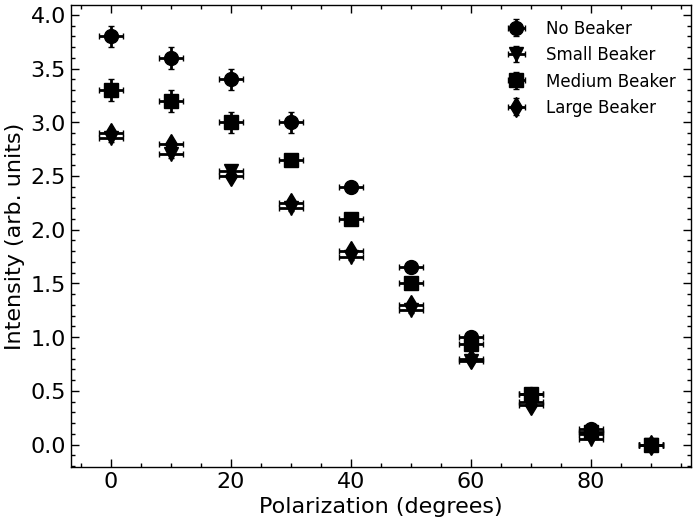
\includegraphics[width=\columnwidth]{../figures/no_water.png}
    \end{center}
    \caption{Intensity vs. Polarization for varying beaker sizes with no water. Here, the polarization is measured in degrees and the intensity is measured in arbitrary units.}
    \label{fig:no_water}
\end{figure}

\begin{figure}[H]
    \begin{center}
        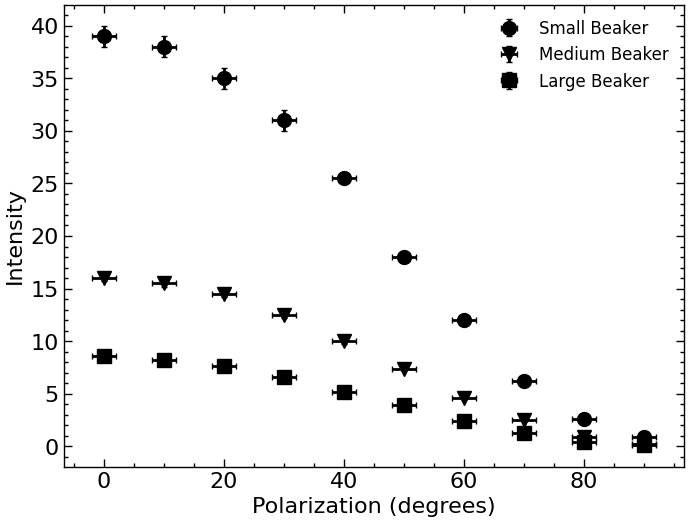
\includegraphics[width=\columnwidth]{../figures/water.png}
    \end{center}
    \caption{Intensity vs. Polarization for varying beaker sizes with water. Here, the polarization is measured in degrees and the intensity is measured in arbitrary units.}
    \label{fig:water}
\end{figure}

\begin{figure}[H]
    \begin{center}
        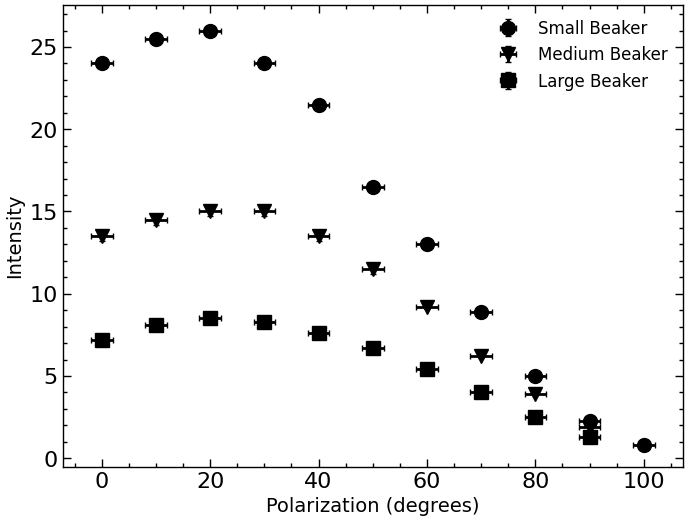
\includegraphics[width=\columnwidth]{../figures/solution1.png}
    \end{center}
    \caption{Intensity vs. Polarization for varying beaker sizes with solution 1. Here, the polarization is measured in degrees and the intensity is measured in arbitrary units.}
    \label{fig:solution1}
\end{figure}

\begin{figure}[H]
    \begin{center}
        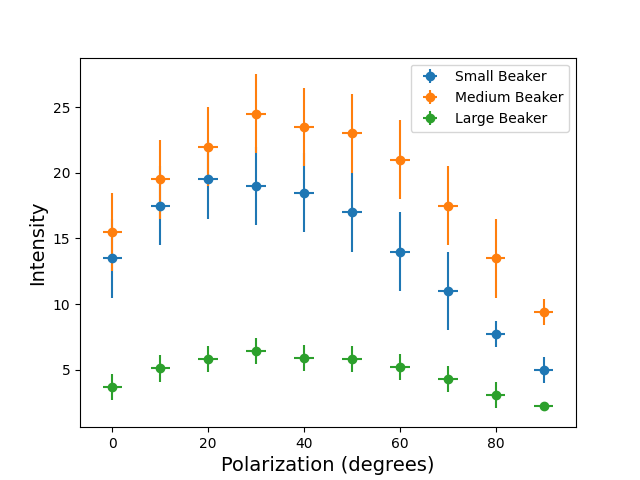
\includegraphics[width=\columnwidth]{../figures/solution2.png}
    \end{center}
    \caption{Intensity vs. Polarization for varying beaker sizes with solution 2. Here, the polarization is measured in degrees and the intensity is measured in arbitrary units.}
    \label{fig:solution2}
\end{figure}

\begin{figure}[H]
    \begin{center}
        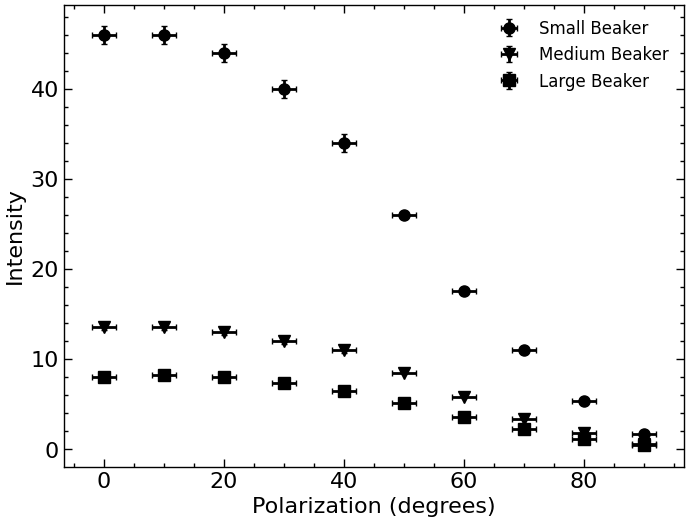
\includegraphics[width=\columnwidth]{../figures/solution3.png}
    \end{center}
    \caption{Intensity vs. Polarization for varying beaker sizes with solution 3. Here, the polarization is measured in degrees and the intensity is measured in arbitrary units.}
    \label{fig:solution3}
\end{figure}

\begin{figure}[H]
    \begin{center}
        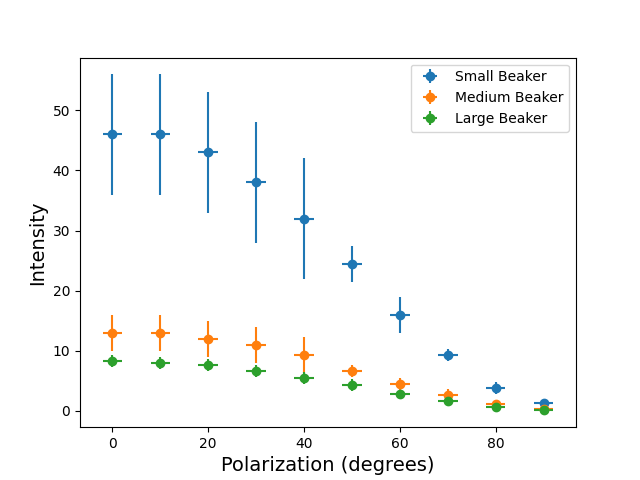
\includegraphics[width=\columnwidth]{../figures/solution4.png}
    \end{center}
    \caption{Intensity vs. Polarization for varying beaker sizes with solution 4. Here, the polarization is measured in degrees and the intensity is measured in arbitrary units.}
    \label{fig:solution4}
\end{figure}

\newpage
Each of the following graphs show the phase shift as a function of sugar concentration in water, with each separate graph containing data from one beaker size. 
The phase shifts were found by fitting the intensity vs. polarization data to a cosine function in the form $A\cos{\left(Bx+C\right)}+D$. We invoked the ODR (orthogonal distance regression) class from the SciPy Python package to fit these data sets to the previously mentioned cosine function. By representing phase shift versus sugar concentration, we can quantify how the polarization of light changes as a function of sugar concentration in water.

\begin{figure}[H]
    \begin{center}
        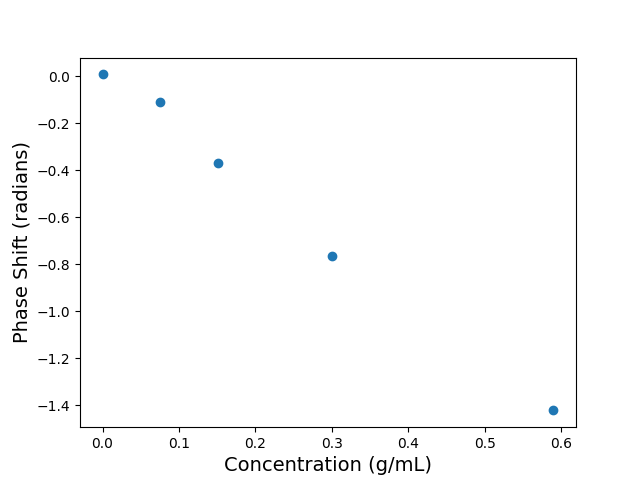
\includegraphics[width=\columnwidth]{../figures/large_beaker_phase_shifts.png}
    \end{center}
    \caption{This graph shows the phase shifts for the large beaker.}
    \label{fig:large_beaker_phase_shifts}
\end{figure}

\begin{figure}[H]
    \begin{center}
        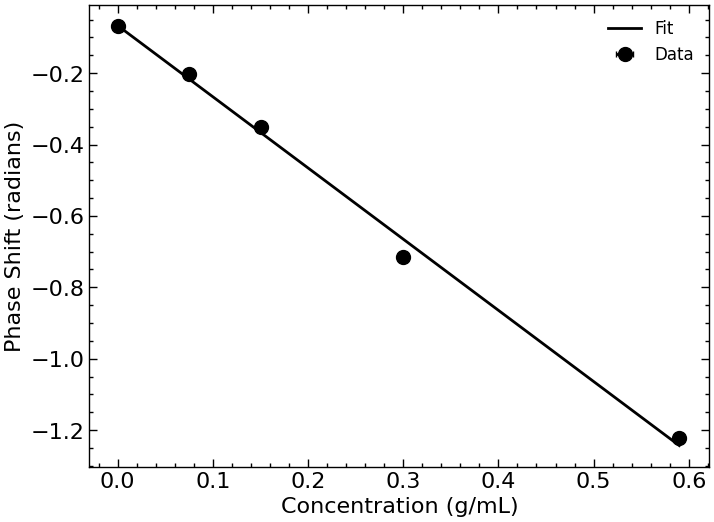
\includegraphics[width=\columnwidth]{../figures/medium_beaker_phase_shifts.png}
    \end{center}
    \caption{Phase shifts for medium beaker.}
    \label{fig:medium_beaker_phase_shifts}
\end{figure}

\begin{figure}[H]
    \begin{center}
        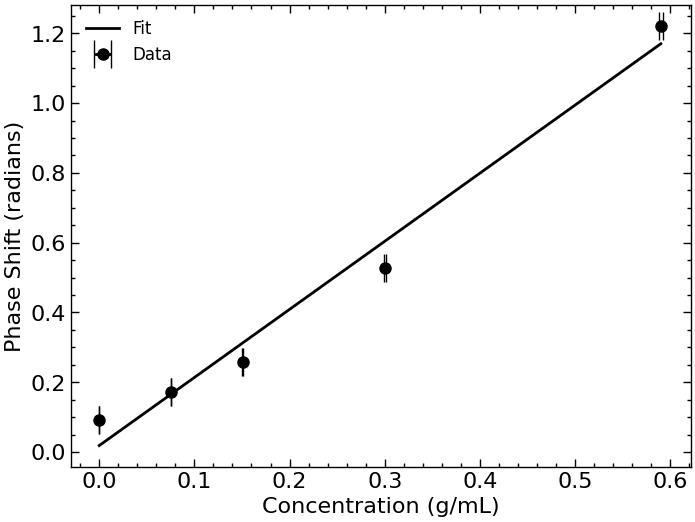
\includegraphics[width=\columnwidth]{../figures/small_beaker_phase_shifts.png}
    \end{center}
    \caption{Phase shifts for small beaker.}
    \label{fig:small_beaker_phase_shifts}
\end{figure}

\begin{figure}[H]
	\begin{center}
		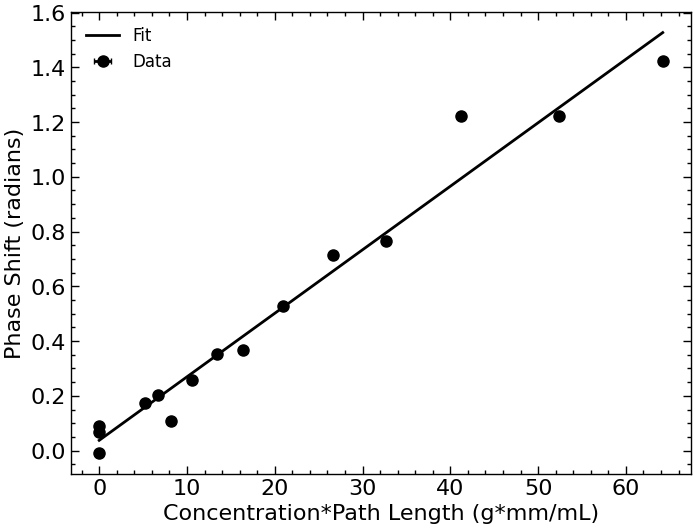
\includegraphics[width=\columnwidth]{../figures/concentration_times_diameter_phase_shifts.png}
	\end{center}
	\caption{This figure encapsulates the phase shift in radians as a function of both concentration in grams per milileter and the path length in milimeters, where the horizontal axis is the product of the concentration and path length values.}
	\label{fig:concentration_times_diameter_phase_shifts}
\end{figure}

\section{Conclusion}
%% Notes
% Important results summarized in a breif and very specific (quantitative) manner.
% Thoughts for future experiments or improvements to the current experiment.


% Important results
Both the concentration of the solution and the path length (distance which the light travels through the solution) affect the polarization of light. The phase shift of the light as a function of the concentration and path length is given by the following equation (extracted from Figure \ref{fig:concentration_times_diameter_phase_shifts}):
\begin{equation}
\phi = 0.02319773(M*L) + 0.03743414,
\end{equation}
where $\phi$ is the phase shift in radians, M is the concentration in grams per milliliter, and L is the path length in millimeters. This equation was obtained by fitting the data to a linear function using the "numpy" polyfit function. Therefore, we found that the phase shift changes at a rate of $0.02319773$ radians per gram millimeter per milliliter. It should also be noted that the R$^2$ of \ref{fig:concentration_times_diameter_phase_shifts} is $0.970$, leading us to belive that phase shift as a function of sugar concentration times path length of light is linear. This result agrees with the previously mentioned paper by K. Sofjan Firdausi et al, where it was shown that the change in polarization as a function of sugar concentration in solution is linear\cite{Firsdausi2018}.

% Thoughts for future experiments or improvements to the current experiment

    
\bibliography{apssamp}% Produces the bibliography via BibTeX.

\end{document}